\chapter{Preface}

\begin{figure}[h]
\begin{minipage}{\textwidth}
\begin{center}
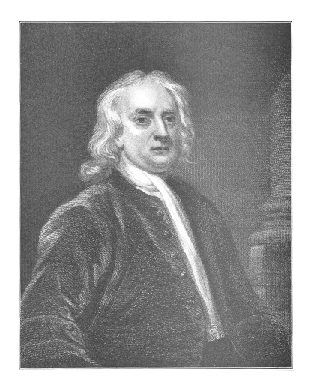
\includegraphics[height=5cm,width=4cm]{images/isaac-newton.eps}
\end{center}
\end{minipage}
\caption{Sir Isaac Newton.}
\label{fig:newton}
\end{figure}

That teachers and students of the Calculus have shown such a 
generous appreciation of Granville's ``Elements of the Differential 
and Integral Calculus'' has been very gratifying to the author. 
In the last few years considerable progress has been made in the 
teaching of the elements of the Calculus, and in this revised 
edition of Granville's ``Calculus'' the latest and best methods 
are exhibited,---methods that have stood the test of actual 
classroom work. Those features of the first edition which 
contributed so much to its usefulness and popularity have been 
retained. The introductory matter has been cut down somewhat in 
order to get down to the real business of the Calculus sooner. 
As this is designed essentially for a drill book, the pedagogic 
principle that each result should be made intuitionally as well 
as analytically evident to the student has been kept constantly 
in mind. The object is not to teach the student to rely on his 
intuition, but, in some cases, to use this faculty in advance 
of analytical investigation. Graphical illustration has been 
drawn on very liberally.

This Calculus is based on the method of limits and is divided 
into two main parts,---Differential Calculus and Integral Calculus. 
As special features, attention may be called to the effort to make 
perfectly clear the nature and extent of each new theorem, the 
large number of carefully graded exercises, and the summarizing 
into working rules of the methods of solving problems. In the 
Integral Calculus the notion of integration over a plane area has 
been much enlarged upon, and integration as the limit of a 
summation is constantly emphasized. The existence of the limit $e$ 
has been assumed and its approximate value calculated from its graph. 
A large number of new examples have been added, both with and without 
answers. At the end of almost every chapter will be found a collection 
of miscellaneous examples. Among the new topics added are approximate 
integration, trapezoidal rule, parabolic rule, orthogonal trajectories, 
centers of area and volume, pressure of liquids, work done, etc. Simple 
practical problems have been added throughout; problems that illustrate 
the theory and at the same time are of interest to the student. These 
problems do not presuppose an extended knowledge in any particular 
branch of science, but are based on knowledge that all students of the 
Calculus are supposed to have in common.

The author has tried to write a textbook that is thoroughly modern and 
teachable, and the capacity and needs of the student pursuing a first 
course in the Calculus have been kept constantly in mind. The book 
contains more material than is necessary for the usual course of one 
hundred lessons given in our colleges and engineering schools; but 
this gives teachers an opportunity to choose such subjects as best 
suit the needs of their classes. It is believed that the volume 
contains all topics from which a selection naturally would be made 
in preparing students either for elementary work in applied science 
or for more advanced work in pure mathematics.

\vskip .3in

\hskip 2in
WILLIAM A. GRANVILLE

\hskip 2in
Gettysburg, Pa.

\begin{figure}[h]
\begin{minipage}{\textwidth}
\begin{center}
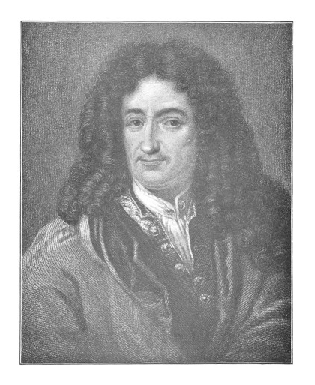
\includegraphics[height=5cm,width=4cm]{images/gottfried-wilhelm-leibnitz.eps}
\end{center}
\end{minipage}
\caption{Gottfried Wilhelm Leibnitz.}
\label{fig:leibnitz}
\end{figure}
